% Graphical abstract, landscape (22 November 2026).
% Canvas 160 mm x 112 mm (1.43:1, the shape of the publisher's landscape examples); x = y = 1 mm, origin at the
% top left, y downward. Smallest text 7 pt at this size; the one exponent (13) is set at 6 pt.
% Every element is drawn here in TikZ: no bitmap, no generated image, no publisher logo or wordmark.
% Layout: headline bar; three panels with coloured header bars (what the system does, x 3-51.5; what was measured,
% x 54.5-116.5; limits, x 119.5-157; all y 18.5-93); a line defining the abbreviations; a takeaway bar.
% The two latency tiles have the same size, layout and type sizes, so neither value outweighs the other. Each tile
% gives its set-up before its value, and a gap with a solid rule separates the tiles (separate experiments).
% Every number and statement, with its source in the manuscript:
%   headline   chosen by the corresponding author (22 November 2026).
%   roles      Section "System Overview and Actors" and the application scenario: issuer = platform, holder = user,
%              verifier = relying party; the Issuer signs the VC, the Holder presents it without holder binding.
%   registry   DIDRegistry contract on Ethereum holds DID records and revocation records (Section 4.1, 4.3);
%              the issuer DID's controller registers and revokes; the holder registers the subject DID
%              (Figure 1: createDID for the subject DID); the verifier makes four contract reads at the block
%              selected at B0 (Section 4.5; verifier-service.js 152-224), read-only, no transaction.
%   2.77 ms    pooled median of 100 local in-process verifications, 9 November 2026 (Table 4; abstract; C5).
%              "The EVM ran in-process without a network round trip" (Section 6.3).
%   616.6 ms   pooled median of 100 Sepolia verifications in ten windows, 12 November 2026, one client on a mobile
%              hotspot through one RPC provider (Table 5, P; abstract; C5). Separate experiment (abstract; C5):
%              the two values are not compared and no ratio is shown; the Sepolia
%              time includes the round trips to the RPC provider.
%   gas        Table 3, 9 November 2026: register subject DID 466,991 (local, Osaka) and 2,139,071 (Sepolia,
%              Glamsterdam); revoke one credential 56,791 and 138,811.
%   164 tests  Section 6.4 and Table 6: the suite of 164 tests passes at the archived commit 73b4cca16e7c.
%   limits     no holder binding (Section 4.1; also at the presents arrow); administrators can pause
%              registration, key rotation and document changes for every DID, while revocation and deactivation stay
%              available (abstract; Section 4.6.2); about 4.7 x 10^13 gas for one hundred million
%              holder registrations under the mainnet (Osaka) schedule, by extrapolation (abstract; Section 8.6).
%   reads      the dashed read arrow ends between the DID records and the revocation records: three of the four
%              reads (verifyDID twice, getDIDDocument) read DID records, one (isCredentialRevoked) revocation records.
%   takeaway   Conclusion (holder binding is stated at the arrow and under Limits, not repeated here).
%   abbreviations as in the paper's list of abbreviations.
% Colours: navy, teal and maroon header bars; Okabe-Ito sky (#56B4E9, line #2E86B8) for DID records and
% vermilion (#D55E00 fills, lines and icon, #B34700 for the "revoke VC" label) for revocation, as in Figure 1; the
% "revocation records" label is black for contrast; green for the test result. Dashed lines only for the read-only
% query; the separators in the Limits panel are solid #BFBFBF rules.
% Font: Helvetica (URW Nimbus Sans, Type 1, embedded).
% Build: see build_all.sh (pdflatex, then pdftoppm -r 600 for the PNG and Pillow for the TIFF).
\documentclass[border=0pt]{standalone}
\usepackage[T1]{fontenc}
\usepackage{textcomp}
\usepackage[scaled=1]{helvet}
\renewcommand{\familydefault}{\sfdefault}
\usepackage{tikz}
\usetikzlibrary{arrows.meta, calc}
\pdfinfoomitdate=1 \pdftrailerid{} \pdfsuppressptexinfo=-1

% Palette
\definecolor{navy}{HTML}{1B3A5C}
\definecolor{teal}{HTML}{0E6B70}
\definecolor{maroon}{HTML}{7A1F3D}
\definecolor{okgreen}{HTML}{1E7A4C}
\definecolor{oisky}{HTML}{56B4E9}
\definecolor{skyline}{HTML}{2E86B8}
\definecolor{oiverm}{HTML}{D55E00}
\definecolor{vtext}{HTML}{B34700}
\definecolor{greytext}{HTML}{404040}
\definecolor{pagebg}{HTML}{F3F5F8}
\definecolor{tilebg}{HTML}{EEF2F7}
\definecolor{rulegrey}{HTML}{BFBFBF}

\newcommand{\fs}[1]{\fontsize{#1}{1.2\dimexpr#1pt\relax}\selectfont}
\newcommand{\tms}{\,\texttimes\,}

% ---------- Icons (drawn about the origin, y downward, sizes in mm) ----------
% Platform: a building with windows.
\newcommand{\iconbuilding}[3]{%
  \begin{scope}[shift={(#1,#2)}]
    \fill[#3] (-3.4,-3.0) rectangle (3.4,4.0);
    \fill[#3] (-2.4,-4.0) rectangle (2.4,-3.0);
    \foreach \cx in {-2.3,-0.5,1.3} \foreach \cy in {-2.2,-0.4,1.4}
      \fill[white] (\cx,\cy) rectangle ++(1.0,1.0);
    \fill[white] (-0.7,2.9) rectangle (0.7,4.0);
  \end{scope}}
% User: a person holding a phone (wallet).
\newcommand{\iconuser}[3]{%
  \begin{scope}[shift={(#1,#2)}]
    \fill[#3] (-0.9,-2.3) circle (1.7);
    \fill[#3, rounded corners=1.5mm] (-4.0,4.6) rectangle (2.2,0.2);
    \fill[pagebg] (-4.2,4.0) rectangle (2.4,4.8);
    \fill[teal, draw=white, line width=0.35mm, rounded corners=0.45mm] (1.0,-0.6) rectangle (3.9,4.0);
    \fill[white] (1.55,0.1) rectangle (3.35,2.9);
  \end{scope}}
% Relying party: a shield with a tick.
\newcommand{\iconshield}[3]{%
  \begin{scope}[shift={(#1,#2)}]
    \fill[#3] (0,-4.0) -- (3.4,-2.8) -- (3.4,0.0) .. controls (3.4,2.3) and (1.8,3.5) .. (0,4.3)
              .. controls (-1.8,3.5) and (-3.4,2.3) .. (-3.4,0.0) -- (-3.4,-2.8) -- cycle;
    \draw[white, line width=0.6mm, line cap=round, line join=round] (-1.6,0.1) -- (-0.4,1.4) -- (1.8,-1.4);
  \end{scope}}
% Chain of three blocks.
\newcommand{\iconchain}[3]{%
  \begin{scope}[shift={(#1,#2)}]
    \foreach \bx in {-6.2,-1.6,3.0} {
      \fill[#3!55] (\bx,-1.2) -- (\bx+0.8,-2.0) -- (\bx+3.6,-2.0) -- (\bx+2.8,-1.2) -- cycle;
      \fill[#3!80] (\bx+2.8,-1.2) -- (\bx+3.6,-2.0) -- (\bx+3.6,0.8) -- (\bx+2.8,1.6) -- cycle;
      \fill[#3] (\bx,-1.2) rectangle (\bx+2.8,1.6);
    }
    \draw[#3, line width=0.35mm] (-3.4,0.2) -- (-1.6,0.2) (1.2,0.2) -- (3.0,0.2);
  \end{scope}}
% Key.
\newcommand{\iconkey}[3]{%
  \begin{scope}[shift={(#1,#2)}]
    \draw[#3, line width=0.55mm] (-2.2,0) circle (1.25);
    \draw[#3, line width=0.55mm, line cap=round] (-0.95,0) -- (3.2,0) (2.3,0) -- (2.3,1.2) (3.2,0) -- (3.2,1.4);
  \end{scope}}
% Revoked certificate: a page with lines and a cross badge.
\newcommand{\iconrevoked}[3]{%
  \begin{scope}[shift={(#1,#2)}]
    \fill[white, draw=#3, line width=0.35mm] (-2.4,-2.8) -- (1.0,-2.8) -- (2.2,-1.6) -- (2.2,2.8) -- (-2.4,2.8) -- cycle;
    \draw[#3, line width=0.3mm] (-1.6,-1.2) -- (0.6,-1.2) (-1.6,0) -- (1.4,0) (-1.6,1.2) -- (0.4,1.2);
    \fill[#3] (1.9,2.0) circle (1.45);
    \draw[white, line width=0.38mm, line cap=round] (1.25,1.35) -- (2.55,2.65) (1.25,2.65) -- (2.55,1.35);
  \end{scope}}
% Laptop.
\newcommand{\iconlaptop}[3]{%
  \begin{scope}[shift={(#1,#2)}]
    \fill[#3, rounded corners=0.4mm] (-3.0,-2.4) rectangle (3.0,1.6);
    \fill[white] (-2.4,-1.8) rectangle (2.4,1.0);
    \fill[#3] (-4.0,2.0) -- (4.0,2.0) -- (3.4,2.9) -- (-3.4,2.9) -- cycle;
    \draw[#3, line width=0.3mm, line cap=round, line join=round]
      (-0.9,-1.15) -- (-1.75,-0.4) -- (-0.9,0.35) (0.9,-1.15) -- (1.75,-0.4) -- (0.9,0.35) (0.35,-1.35) -- (-0.35,0.55);
  \end{scope}}
% Phone with hotspot signal, and a cloud for the remote network.
\newcommand{\iconhotspot}[3]{%
  \begin{scope}[shift={(#1,#2)}]
    \fill[#3, rounded corners=0.45mm] (-1.3,-0.6) rectangle (1.3,4.0);
    \fill[white] (-0.85,0.0) rectangle (0.85,3.0);
    \foreach \r in {1.6,2.6,3.6}
      \draw[#3, line width=0.32mm, line cap=round] (0,-1.0) ++(235:\r) arc[start angle=235, end angle=305, radius=\r];
  \end{scope}}
% Fuel pump (gas).
\newcommand{\iconpump}[3]{%
  \begin{scope}[shift={(#1,#2)}]
    \fill[#3, rounded corners=0.3mm] (-2.0,-2.4) rectangle (1.0,2.6);
    \fill[white] (-1.4,-1.8) rectangle (0.4,-0.4);
    \draw[#3, line width=0.35mm, line cap=round, line join=round] (1.0,-0.6) -- (2.0,0.2) -- (2.0,1.8) -- (2.6,1.8) -- (2.6,-1.4);
  \end{scope}}
% Tick in a circle.
\newcommand{\icontick}[3]{%
  \begin{scope}[shift={(#1,#2)}]
    \fill[#3] (0,0) circle (2.0);
    \draw[white, line width=0.45mm, line cap=round, line join=round] (-0.95,0.05) -- (-0.25,0.8) -- (1.05,-0.75);
  \end{scope}}
% Badged icons for the limits panel: #1 a named coordinate (badge centre), #2 colour.
\newcommand{\badge}[2]{\fill[#2!10, draw=#2, line width=0.3mm] (#1) circle (3.3);}
% Broken link.
\newcommand{\iconbroken}[2]{%
  \badge{#1}{#2}
  \begin{scope}[shift={(#1)}, rotate=-45]
    \draw[#2, line width=0.45mm, rounded corners=0.6mm] (-2.6,-0.75) rectangle (-0.5,0.75);
    \draw[#2, line width=0.45mm, rounded corners=0.6mm] (0.5,-0.75) rectangle (2.6,0.75);
  \end{scope}
  \begin{scope}[shift={(#1)}]
    \draw[#2, line width=0.3mm, line cap=round] (-0.9,0.15) -- (-0.4,0.55) (0.4,-0.55) -- (0.9,-0.15);
  \end{scope}}
% Pause.
\newcommand{\iconpause}[2]{%
  \badge{#1}{#2}
  \begin{scope}[shift={(#1)}]
    \fill[#2] (-1.25,-1.5) rectangle (-0.35,1.5) (0.35,-1.5) rectangle (1.25,1.5);
  \end{scope}}
% Stack of coins.
\newcommand{\iconcoins}[2]{%
  \badge{#1}{#2}
  \begin{scope}[shift={(#1)}]
    \foreach \cy in {1.3,0.3,-0.7} {
      \fill[#2] (-1.7,\cy) rectangle (1.7,\cy+0.6);
      \fill[#2] (0,\cy+0.6) ellipse (1.7 and 0.45);
      \fill[#2!35] (0,\cy) ellipse (1.7 and 0.45);
    }
    \draw[#2, line width=0.2mm] (0,-0.7) ellipse (1.7 and 0.45);
  \end{scope}}
% Target.
\newcommand{\icontarget}[3]{%
  \begin{scope}[shift={(#1,#2)}]
    \fill[white] (0,0) circle (3.2);
    \fill[#3] (0,0) circle (2.4);
    \fill[white] (0,0) circle (1.6);
    \fill[#3] (0,0) circle (0.8);
  \end{scope}}

\begin{document}
\frenchspacing
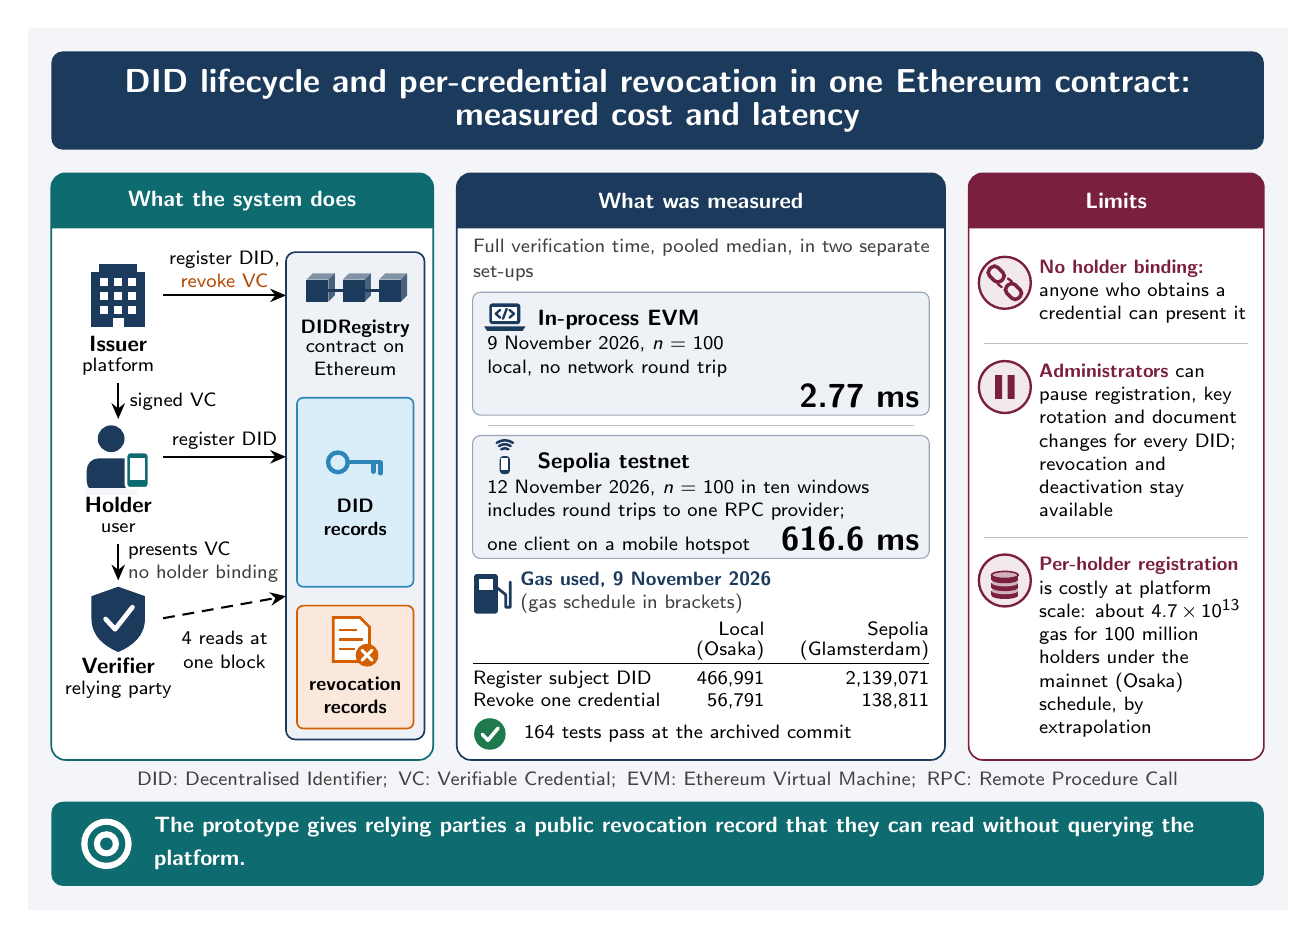
\begin{tikzpicture}[x=1mm, y={(0mm,-1mm)},
    call/.style={-{Stealth[length=2.0mm,width=1.7mm]}, line width=0.75pt},
    read/.style={-{Stealth[length=2.0mm,width=1.7mm]}, line width=0.75pt, dash pattern=on 1.5mm off 1mm},
    lab/.style={inner sep=0pt, align=flush center, font=\fs{7}},
    txt/.style={inner sep=0pt, align=flush left, anchor=north west},
  ]
  \useasboundingbox (0,0) rectangle (160,112);
  \fill[pagebg] (0,0) rectangle (160,112);

  % ---------- Headline bar ----------
  \fill[navy, rounded corners=1.5mm] (3,3) rectangle (157,15.5);
  \node[inner sep=0pt, align=flush center, text=white, text width=150mm] at (80,9.25)
    {\fs{11.5}\bfseries DID lifecycle and per-credential revocation in one Ethereum contract:\\ measured cost and latency};

  % ---------- Panel frames ----------
  % Panels 3-51.5, 54.5-116.5, 119.5-157 (gaps 3 mm); the middle panel is the widest, for the latency tiles and
  % the gas table.
  % #1 x left, #2 x right, #3 colour, #4 title
  \newcommand{\panel}[4]{%
    \fill[white, draw=#3, line width=0.6pt, rounded corners=1.8mm] (#1,18.5) rectangle (#2,93);
    \fill[#3] (#1,25.5) [rounded corners=1.8mm] -- (#1,18.5) -- (#2,18.5) [sharp corners] -- (#2,25.5) -- cycle;
    \node[inner sep=0pt, text=white] at ({(#1+#2)/2},22) {\fs{8.5}\bfseries #4};}
  \panel{3}{51.5}{teal}{What the system does}
  \panel{54.5}{116.5}{navy}{What was measured}
  \panel{119.5}{157}{maroon}{Limits}

  % ---------- Panel 1: roles and registry ----------
  % Role cards (icon, name, descriptor), column centre x = 11.5
  \iconbuilding{11.5}{34}{navy}
  \node[lab] at (11.5,40.1) {\fs{8}\bfseries Issuer};
  \node[lab] at (11.5,43.1) {platform};
  \iconuser{11.5}{54.5}{navy}
  \node[lab] at (11.5,60.6) {\fs{8}\bfseries Holder};
  \node[lab] at (11.5,63.6) {user};
  \iconshield{11.5}{75}{navy}
  \node[lab] at (11.5,81.1) {\fs{8}\bfseries Verifier};
  \node[lab] at (11.5,84.1) {relying party};
  % Credential flow between the roles
  \draw[call] (11.5,45.1) -- (11.5,49.7);
  \node[lab, anchor=west] at (12.9,47.5) {signed VC};
  \draw[call] (11.5,65.6) -- (11.5,70.2);
  \node[lab, anchor=west, align=flush left] at (12.7,67.9) {presents VC\\\textcolor{greytext}{no holder binding}};

  % Registry, column centre x = 41.6 (moved 0.8 mm right so that the grey label clears it). The gap between the two record boxes (y 71-73.4) is level with the end of
  % the dashed read arrow, which reads both kinds of record.
  \fill[tilebg, draw=navy, line width=0.6pt, rounded corners=1.2mm] (32.8,28.5) rectangle (50.4,90.4);
  \iconchain{41.6}{33.2}{navy}
  \node[lab] at (41.6,38.2) {\fs{7.5}\bfseries DIDRegistry};
  \node[lab] at (41.6,42) {contract on\\Ethereum};
  \fill[oisky!22, draw=skyline, line width=0.6pt, rounded corners=0.8mm] (34.2,47) rectangle (49.0,71);
  \iconkey{41.6}{55.2}{skyline}
  \node[lab] at (41.6,62.2) {\fs{7.5}\bfseries DID\\\fs{7.5}\bfseries records};
  \fill[oiverm!14, draw=oiverm, line width=0.6pt, rounded corners=0.8mm] (34.2,73.4) rectangle (49.0,89);
  \iconrevoked{41.2}{77.7}{oiverm}
  \node[lab] at (41.6,84.8) {\fs{7.5}\bfseries revocation\\\fs{7.5}\bfseries records};

  % Calls to the registry: solid = transaction, dashed = read-only query
  \draw[call] (17.2,34) -- (32.8,34);
  \node[lab, anchor=south] at (25.0,33.1) {register DID,\\\textcolor{vtext}{revoke VC}};
  \draw[call] (17.2,54.5) -- (32.8,54.5);
  \node[lab, anchor=south] at (25.0,53.6) {register DID};
  \draw[read] (17.2,75) -- (32.8,72.2);
  \node[lab, anchor=north] at (25.0,76.6) {4 reads at\\one block};

  % ---------- Panel 2: measured ----------
  \node[txt, text width=58mm, font=\fs{7.5}, text=greytext] at (56.5,26.8)
    {Full verification time, pooled median, in two separate set-ups};
  % Two tiles of equal size and the same layout, so the two values have equal weight. Rows (baselines from the tile
  % top T): set-up name at T+4.2; date and n at T+7.3; conditions at T+10.3 (and T+14.6 in the Sepolia tile). The
  % value is the last item of each tile, right-aligned on the bottom row, so each tile states its set-up before its
  % value. A 2.6 mm gap with a solid rule separates the tiles.
  \def\tileh{15.6}
  \newcommand{\tile}[1]{\fill[tilebg, draw=navy!45, line width=0.4pt, rounded corners=1mm] (56.5,#1) rectangle (114.5,#1+\tileh);}
  \def\ta{33.6} \def\tb{51.8}
  \tile{\ta}
  \begin{scope}[shift={(60.6,\ta+3.0)}, scale=0.66]\iconlaptop{0}{0}{navy}\end{scope}
  \node[txt, anchor=base west] at (64.7,\ta+4.2) {\fs{8}\bfseries In-process EVM};
  \node[txt, anchor=base west, font=\fs{7}] at (58.3,\ta+7.3) {9 November 2026, \textit{n} = 100};
  \node[txt, anchor=base west, font=\fs{7}] at (58.3,\ta+10.3) {local, no network round trip};
  \node[inner sep=0pt, anchor=base east] at (113.3,\ta+14.6) {\fs{12}\bfseries 2.77 ms};
  \draw[rulegrey, line width=0.4pt] (58.5,{(\ta+\tileh+\tb)/2}) -- (112.5,{(\ta+\tileh+\tb)/2});
  \tile{\tb}
  \begin{scope}[shift={(60.6,\tb+2.9)}, scale=0.5]\iconhotspot{0}{0}{navy}\end{scope}
  \node[txt, anchor=base west] at (64.7,\tb+4.2) {\fs{8}\bfseries Sepolia testnet};
  \node[txt, anchor=base west, font=\fs{7}] at (58.3,\tb+7.3) {12 November 2026, \textit{n} = 100 in ten windows};
  \node[txt, anchor=base west, font=\fs{7}] at (58.3,\tb+10.3) {includes round trips to one RPC provider;};
  \node[txt, anchor=base west, font=\fs{7}] at (58.3,\tb+14.6) {one client on a mobile hotspot};
  \node[inner sep=0pt, anchor=base east] at (113.3,\tb+14.6) {\fs{12}\bfseries 616.6 ms};

  % Gas (Table 3): title and table. The heads "Local (Osaka)" and "Sepolia (Glamsterdam)" need about 65 mm on one line
  % next to the row labels, more than the 58 mm of the panel, so each head breaks once, before its bracket.
  \iconpump{58.7}{71.8}{navy}
  \node[txt, anchor=base west] at (62.5,70.8) {\fs{7.5}\bfseries\color{navy} Gas used, 9 November 2026};
  \node[txt, anchor=base west] at (62.5,73.8) {\fs{7}\color{greytext}(gas schedule in brackets)};
  \node[txt] at (56.5,75.2) {\fs{7}\setlength{\tabcolsep}{2.25mm}\renewcommand{\arraystretch}{0.95}%
    \begin{tabular}{@{}l r r@{}}
      & Local & Sepolia\\[-0.35mm]
      & (Osaka) & (Glamsterdam)\\[0.2mm]
      \hline\noalign{\vskip 0.6mm}
      Register subject DID & 466,991 & 2,139,071\\
      Revoke one credential & 56,791 & 138,811
    \end{tabular}};

  % Tests
  \icontick{58.7}{89.7}{okgreen}
  \node[txt, anchor=west] at (62.1,89.7) {\fs{7.5} 164 tests pass at the archived commit};

  % ---------- Panel 3: limits ----------
  % The first item starts below the header bar, the last ends above the panel's bottom edge, and the middle item is
  % centred between them, so the two gaps are equal; each separator sits in the middle of its gap.
  \node[txt, text width=27.4mm, font=\fs{7}] (L1) at (128.4,29.4)
    {\textbf{\color{maroon}No holder binding:} anyone who obtains a credential can present it};
  \node[txt, text width=27.4mm, font=\fs{7}, anchor=south west] (L3) at (128.4,90.2)
    {\textbf{\color{maroon}Per-holder registration} is costly at platform scale: about 4.7\tms10\raisebox{0.85ex}{\fs{6}13} gas for 100 million holders under the mainnet (Osaka) schedule, by extrapolation};
  \node[txt, text width=27.4mm, font=\fs{7}, anchor=west] (L2) at ($(L1.south west)!0.5!(L3.north west)$)
    {\textbf{\color{maroon}Administrators} can pause registration, key rotation and document changes for every DID; revocation and deactivation stay available};
  \foreach \i in {1,2,3} \coordinate (B\i) at ($(L\i.north west)+(-4.3,3.0)$);
  \iconbroken{B1}{maroon}
  \iconpause{B2}{maroon}
  \iconcoins{B3}{maroon}
  \coordinate (S1) at ($(L1.south)!0.5!(L2.north)$);
  \coordinate (S2) at ($(L2.south)!0.5!(L3.north)$);
  \foreach \s in {S1,S2}
    \draw[rulegrey, line width=0.3pt] (121.5,0 |- \s) -- (155,0 |- \s);

  % ---------- Abbreviations ----------
  \node[inner sep=0pt] at (80,95.6)
    {\fs{7}\color{greytext} DID: Decentralised Identifier;\enspace VC: Verifiable Credential;\enspace EVM: Ethereum Virtual Machine;\enspace RPC: Remote Procedure Call};

  % ---------- Takeaway bar ----------
  \fill[teal, rounded corners=1.5mm] (3,98.3) rectangle (157,109);
  \icontarget{10}{103.65}{teal}
  \node[inner sep=0pt, align=flush left, text=white, text width=138mm, anchor=west] at (16,103.65)
    {\fs{8.5}\bfseries The prototype gives relying parties a public revocation record that they can read without querying the platform.};
\end{tikzpicture}
\end{document}
